\chapter{Related Works}

Your related works, and your purpose and contribution which must be different as below.

\section{Aip Suprapto Munari/1164063}
\subsection{Teori}
\subsection{Binary Classification}
\begin{enumerate}
\item Binary Classification atau diartikan kedalam bahasa indonesia yaitu Klasifikasi Biner adalah tugas dalam mengkalrifikasikan elemen-elemen dari himpunan yang diberikan kedalam dua kelompok berdasarkan aturan klarifikasi. Pada ummnya klarifikasi biner akan jatuh ke dalam domain Supervised Learning dan dimana kasus khusus hanya memiliki dua kelas. Beberapa contoh yang meliputi Binary Classification adalah \begin{itemize}
		\item Deteksi Transaksi Penipuan Kartu Kredit
		\item Diagnosa medis
		\item Deteksi Spam
	\end{itemize}
\subitem Untuk contoh Binary Classification dapat dilihat pada gambar \ref{YNBC}
		\begin{figure}[ht]
		\centerline{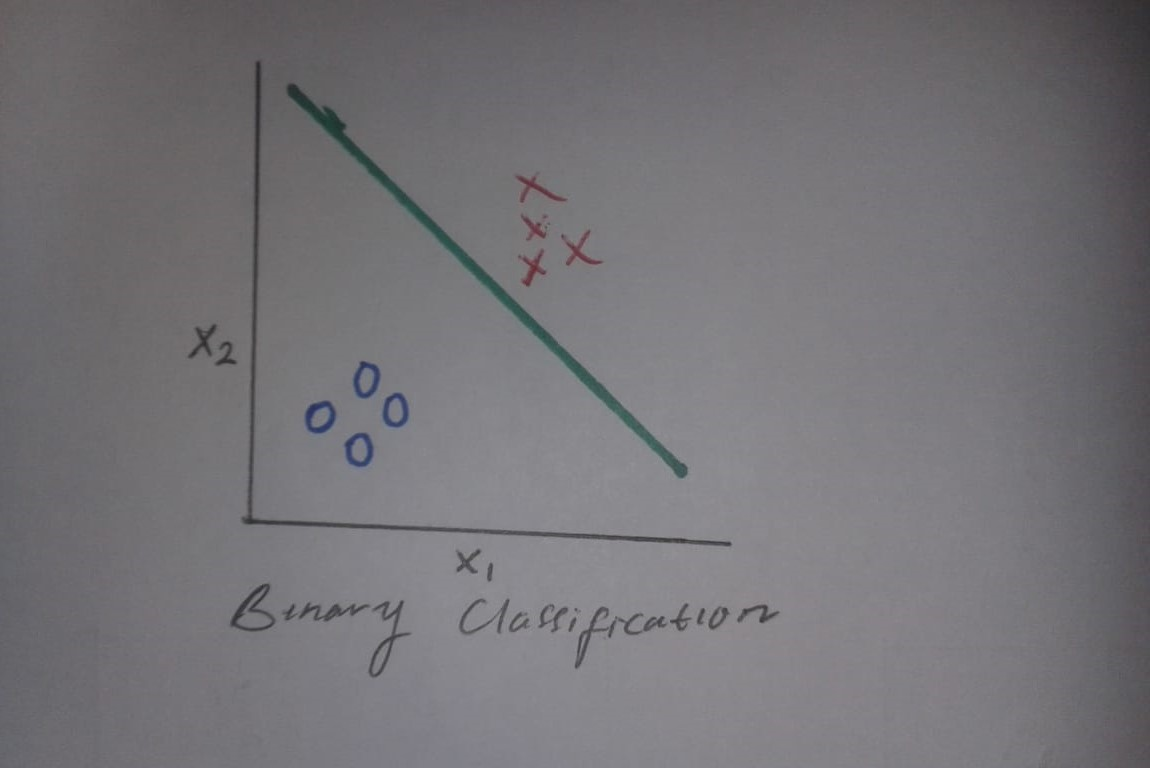
\includegraphics[width=1\textwidth]{figures/AIP/1.JPEG}}
		\caption{Binary Classification.}
		\label{1}
		\end{figure}
 \end{enumerate}

\subsection{Supervised Learning, Unsupervised Learning, Dan Classtering}
\begin{enumerate}
\item Supervised Learning merupakan sebuah pendekatan yang dimana sudah adanya sdata yang dilatih dan telah terdapat variabel yang telah ditargetkan sehingga bertujuan untuk mengelompokkan suatu data ke data yang sudah ada. Contoh dalam Supervised Learning yaitu ketika anda memiliki sejumlah buku yang yang telah dilabel dengan urutan kategori tertentu. Ketika anda akan membeli sebuah buku baru, maka harus di identifikasi isi dari buku tersebut dan memasukkannya kedalam kategori tertentu. Ketika anda membeli sebuah buku tersebut maka anda telah menerapkan sebuah logika fuzzy. Ilustrasi Supervised Learning dapat dilihat pada gambar \ref{YNSL}.

		\begin{figure}[ht]
		\centerline{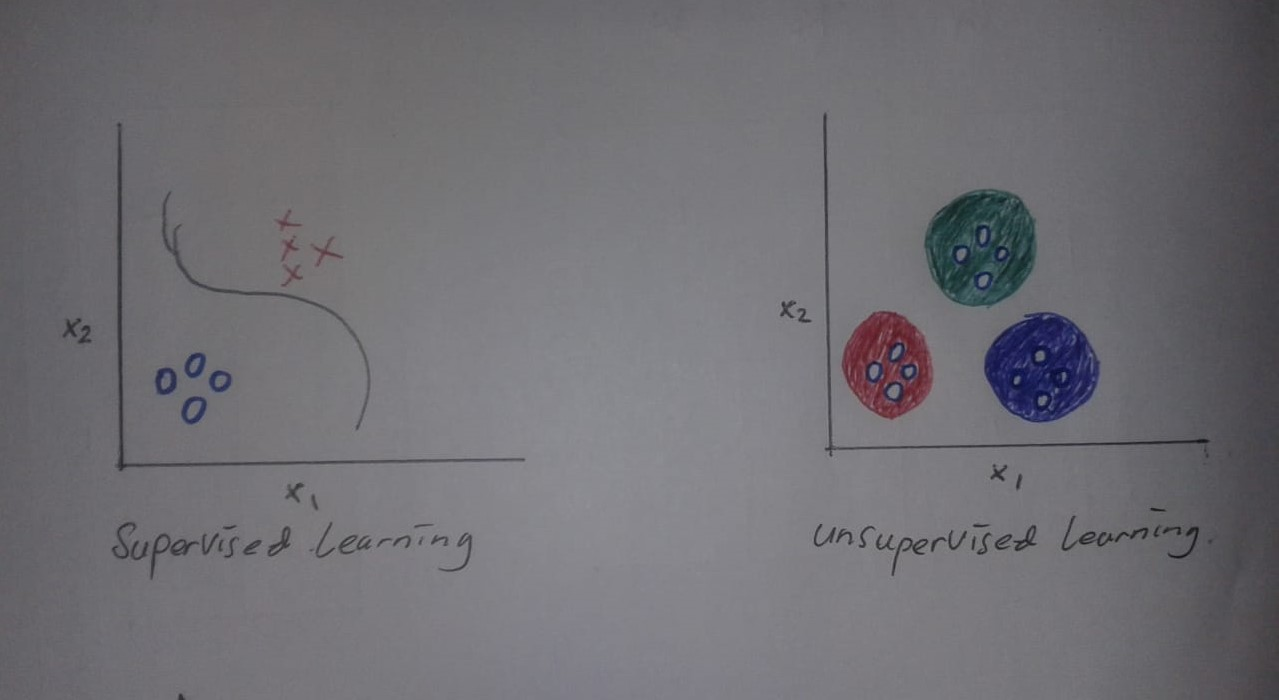
\includegraphics[width=1\textwidth]{figures/AIP/2.JPEG}}
		\caption{Supervised Learning.}
		\label{2}
		\end{figure}

\item Unsupervised Learning merupakan sebuah data yang belum ditentukan variabelnya jadi hanya berupa data saja. Dalam sebuah kasus Unsupervised Learning adalah aggap saja anda belum pernah membeli buku sama sekali dan pada suatu hari anda telah membeli buku dengan sangat banyak dalam kategori yang berbeda. Sehingga buku tersebut belum di kategorikan dan hanya berupa data buku saja. Ilustrasi Unsupervised Learning dapat dilihat pada gambar \ref{YNUSL}.

		\begin{figure}[ht]
		\centerline{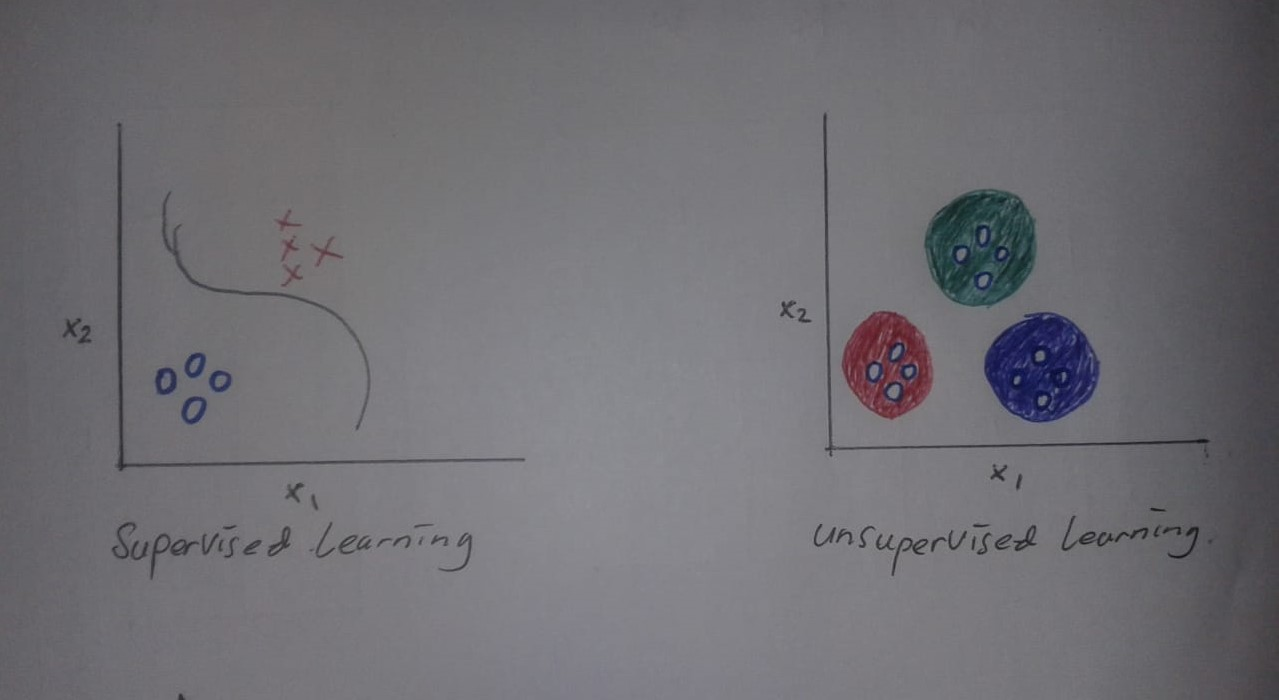
\includegraphics[width=1\textwidth]{figures/AIP/2.JPEG}}
		\caption{Unsupervised Learning.}
		\label{2}
		\end{figure}

\item Classtering merupakan sebuah proses untuk mengklasifikasikan sebuah data dalam satu parameter. Dalam kasus ini dapat dijelaskan ada beberapa orang yang memiliki kekuatan tubuh yang sehat dan kekuatan tubuh yang lemah. Parameter bagi orang yang memiliki tubuh yang kuat adalah orang yang terlihat bugar dan sehat maka dengan orang yang memiliki parameter adalah orang yang memiliki kekuatan tubuh yang kuat dan untuk kekuatan tubuh yang lemah adalah sebaliknya. Ilustrasi gambar dapat di lihat di gambar \ref{YNC}

		\begin{figure}[ht]
		\centerline{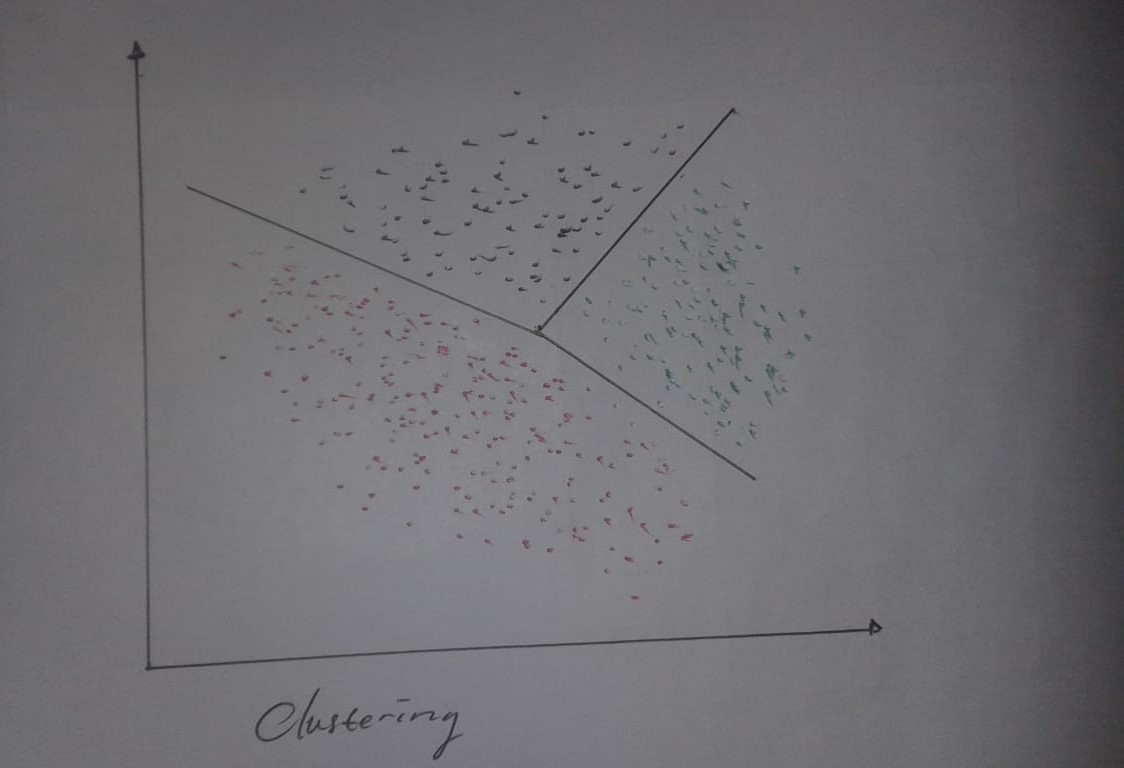
\includegraphics[width=1\textwidth]{figures/AIP/3.JPEG}}
		\caption{Clusterring.}
		\label{3}
		\end{figure}
\end{enumerate}

\subsection{Evaluasi Dan Akurasi}
\begin{enumerate}
\item Evaluasi dan akurasi adalah bagaimana cara kita dapat mengevaluasi sebarapa baik model melakukan pekerjaannya dengan cara mengukur akurasinya. Akurasi akan didefinisikan sebagai presentase kasus yang telah diklasifikasikan dengan benar. Kita dapat melakukan analisis kesalahan yang telah di buat oleh model.Dalam tabel tersebut baris true mangga dan true anggur menunjukkan kasus apakah itu objek mangga atau anggur. Kolom telah di prediksi dan dibuat oleh model. Ada 20 mangga yang di prediksi benar dan ada 5 anggur yang di prediksi salah. Ilustrasi dapat di lihat pada gambar \ref{YEA}

		\begin{figure}[ht]
		\centerline{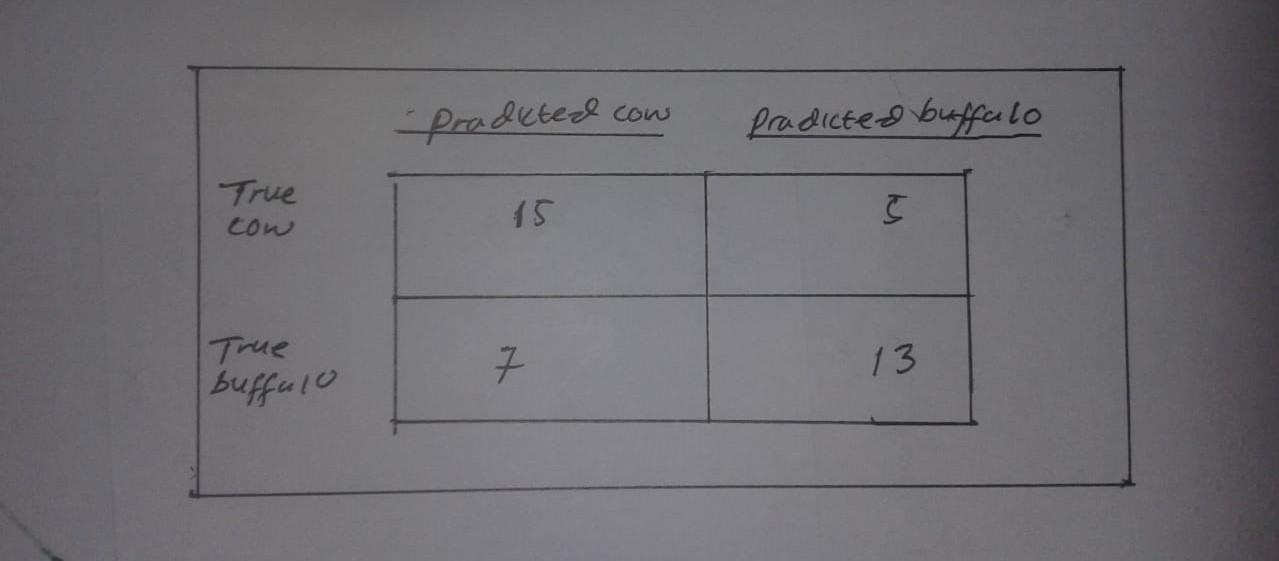
\includegraphics[width=1\textwidth]{figures/AIP/4.JPEG}}
		\caption{Evaluasi Dan Akurasi.}
		\label{4}
		\end{figure}
\end{enumerate}

\subsection{Confusion Matrix}
\begin{enumerate}
\item Ada beberapa cara untuk membuat dan membaca confusion matrix antara lain
	\begin{itemize}
		\item Tentukan pokok permasalahan serta atributnya
		\item Buat Decision Tree
		\item Buat Data Testing
		\item Mencari nilai variabelnya misal a,b,c, dan d
		\item Mencari nilai recall, precision, accuracy, dan erorr rate
	\end{itemize}
\subitem Di bawah ini adalah contoh dari confusion matrix
	\begin{verbatim}
		Recall =3/(1+3) = 0,75
		Precision = 3/(1+3) = 0,75
		Accuracy =(5+3)/(5+1+1+3) = 0,8
		Error Rate =(1+1)/(5+1+1+3) = 0,2 
	\end{verbatim}
\end{enumerate}

\subsection{Cara Kerja K-Fold Cross Validation}
\begin{enumerate}
\item Untuk cara kerja K-Fold Cross Validation adalah sebagai berikut
	\begin{itemize}
		\item Total instance dibagi menjadi N bagian.
		\item Fold yang pertama adalah bagian pertama menjadii testing data dan sisanya menjadi training data.
		\item Hitung akurasi berdasarkan porsi data tersebut dengan menggunakan persamaan.
		\item Fold yang ke dua adalah bagian ke dua menjadi testing data dan sisanya training data. 
		\item Hitung akurasi berdasarkan porsi data tersebut.
		\item Lakukan step secara berulang hingga habis mencapai fold ke-K.
		\item Terakhir hitung rata-rata akurasi K buah.
	\end{itemize}

\subitem Untuk ilustrasi K-Fold Cross Validation data di lihat pada gambar \ref{YNKF}
		\begin{figure}[ht]
		\centerline{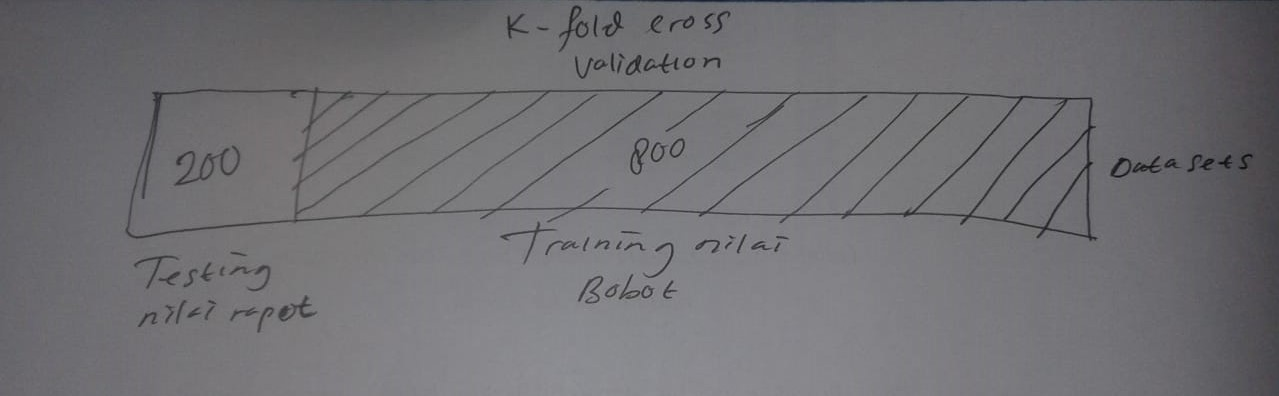
\includegraphics[width=1\textwidth]{figures/AIP/5.JPEG}}
		\caption{K-Fold Cross Validation.}
		\label{5}
		\end{figure}
\end{enumerate}

\subsection{Decision Tree}
\begin{enumerate}
\item Decision Tree adalah sebuah metode pembelajaran yang digunakan untuk melakukan klarifikasi dan regresi. Decision Tree digunakan untuk membuat sebuah model yang dapat memprediksi sebuah nilai variabel target dengan cara mempelajari aturan keputusan dari fitur data. Contoh Decision Tree adalah untuk melakukan predikisi apakah Kuda termasuk hewan mamalia atau bukan, lihat pada gambar \ref{YNDT}.

		\begin{figure}[ht]
		\centerline{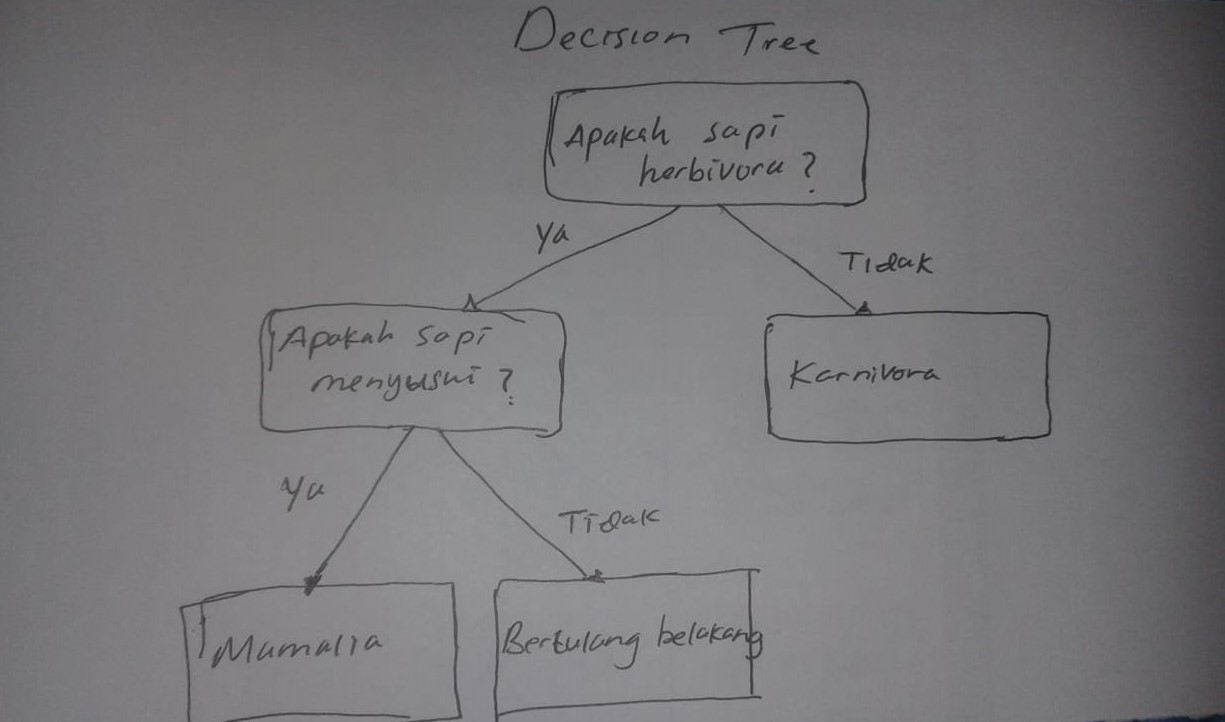
\includegraphics[width=1\textwidth]{figures/AIP/6.JPEG}}
		\caption{Decision Tree.}
		\label{6}
		\end{figure}

\end{enumerate}

\subsection{Gain Dan Entropi}
\begin{enumerate}
\item Gain adalah pengurangan yang diharapkan dalam enthropy. Dalam mechine learning, gain dapat digunakan untuk menentukan sebuah urutan atribut atau memperkecil atribut yang telah dipilih. Urutan ini akan membentuk decision tree. atribut gain dipilih yang paling besar.

\item Entropi adalah ukuran ketidakpastian sebuah variabel acak sehingga dapat di artikan entropi adalah ukuran ketidakpastian dari sebuah atribut.

\subitem Ilustrasi dari gain dan entropi adalah bagaimana kita memprediksi jenis kelamin berdasarkan atributnya, perhatikan pada gambar \ref{YNGE}

		\begin{figure}[ht]
		\centerline{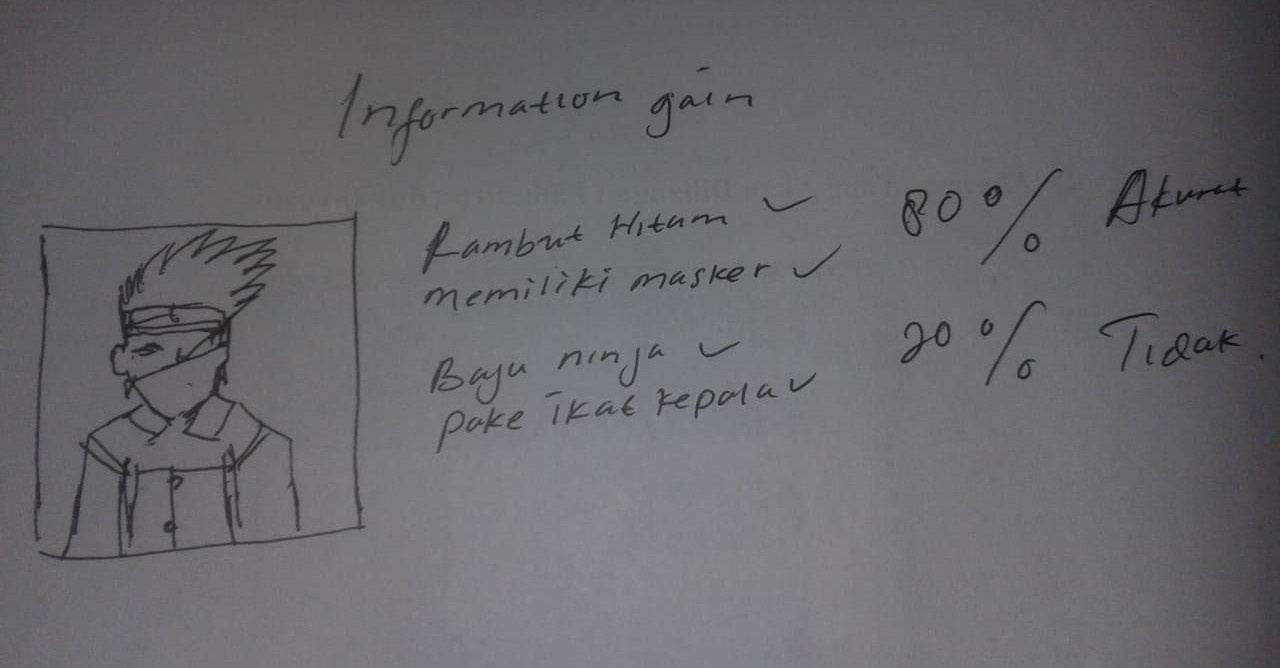
\includegraphics[width=1\textwidth]{figures/AIP/7.JPEG}}
		\caption{Gain Dan Entropi.}
		\label{7}
		\end{figure}
\end{enumerate}


\section{Same Topics}
Cite every latest journal with same topic
\subsection{Topic 1}
cite for first topic

\subsection{Topic 2}
if you have two topics you can include here to


\section{Same Method}
write and cite latest journal with same method

\subsection{Method 1}
cite and paraphrase method 1

\subsection{Method 2}
cite and paraphrase method 2 if you have more method please add new subsection.




 